\documentclass[../../dissertation.tex]{subfiles}
\begin{document}

As was discussed in section \ref{sec:chap3StagWalk}, the elements of each
tessellation of a discretely numbered cycle can be described by states
\begin{equation}
        \ket{\alpha_x} = \frac{\ket{2x} + \ket{2x+1}}{\sqrt{2}},
\end{equation}
\begin{equation}
        \ket{\beta_x} = \frac{\ket{2x+1}+\ket{2x+2}}{\sqrt{2}}.
\end{equation}
These states allow the construction of the Hamiltonians
\begin{equation}
        H_\alpha = 2\sum_{x=-\infty}^{+\infty}\ket{\alpha_{x}}\bra{\alpha_x} - I,
\end{equation}
\begin{equation}
        H_\beta = 2\sum_{x=-\infty}^{+\infty}\ket{\beta_{x}}\bra{\beta_x} - I,
\end{equation}
as in equations \eqref{eq:stagSimulHalpha} and \eqref{eq:stagSimulHbeta}.\par

Following the implementation presented in the work of \cite{acasiete2020},
these operators can be rewritten in matrix form 
\begin{equation}
	H_\alpha = I \otimes X,
\end{equation}
\begin{equation} 
	H_\beta = 
	\begin{pmatrix}
	0 & \cdots & 1\\
	\vdots & H_\alpha & \vdots\\
	1 & \cdots & 0
	\end{pmatrix},
\end{equation} 
which turn out to be very useful representations for the construction of the circuit.\par

As was shown in equation \eqref{eq:stagSimulUniOp}, the unitary evolution
operator is
%TODO: DESCOBRIR SE A OS US ESTAO NA ORDEM CORRETA. 
\begin{equation}
	U = e^{i\theta H_\beta}e^{i\theta H_\alpha} = U_\beta U_\alpha, 
\end{equation} 
knowing that
%TODO: TENTAR DESCOBRIR MELHOR MANEIRA DE REPRESENTAR ISTO. SERA QUE PRECISO DA MATRIZ TODA?  
\begin{equation} 
	R_x(\theta) = e^{\frac{-i\theta X}{2}}, 
\end{equation} 
then each of the evolution operators associated with the different tessellation
Hamiltonians will be 
\begin{equation} 
	U_\alpha = I \otimes R_x(\theta), 
\end{equation}
\begin{equation} 
	U_\beta = 
	\begin{pmatrix}
	\cos{\theta} & \cdots & -i\sin{\theta}\\
	\vdots & U_\alpha & \vdots\\
	-i\sin{\theta}& \cdots & \cos{\theta}
	\end{pmatrix}.
\end{equation}
Notice that $U_\beta$ is simply a permutation of $U_\alpha$, therefore it can
be rewritten as 
\begin{equation}
	U_\beta = P^{-1} U_\alpha P,
\end{equation}
where $P = \sum_x \ket{x+1}\bra{x}$. 
\begin{figure}[!h]
	\[ \Qcircuit @C=1em @R=0.7em {   & & && \mbox{Repeat for steps} & &\\ \\
	               &       & \qw & {/^{\otimes n-1}}\qw      & \multigate{1}{\mbox{INCR}}&\qw &  \multigate{1}{\mbox{DECR}} & \qw \\
            	   &       &\qw & \gate{R_x(2\theta)}    & \ghost{INCR} &\gate{R_x(2\theta)}        & \ghost{DECR} & \qw \gategroup{3}{4}{4}{7}{.8em}{--}
		          } \]
	\caption{General circuit for the staggered quantum walk.}
	\label{fig:stagQWCirc}
\end{figure}\par
Remember from equation \eqref{eq:shiftMatrixQiskit} and figure
\ref{fig:douglasWangShift} that these permutation operators can be implemented
as increment and decrement gates, defined in the work of \cite{douglaswang07}.
Therefore, the circuit for the staggered quantum walk on the line can be
built as shown in figure \ref{fig:stagQWCirc}.\par 

The next step is to implement the circuit in Qiskit, in order to test it in a
real quantum computer. Here, the walk will take place in a cyclic graph with
$8$ elements, which means that 3 qubits will be required, as shown in figure
\ref{fig:stagQWCircuitQistkit}.
\begin{figure}[!h]
	\centering
	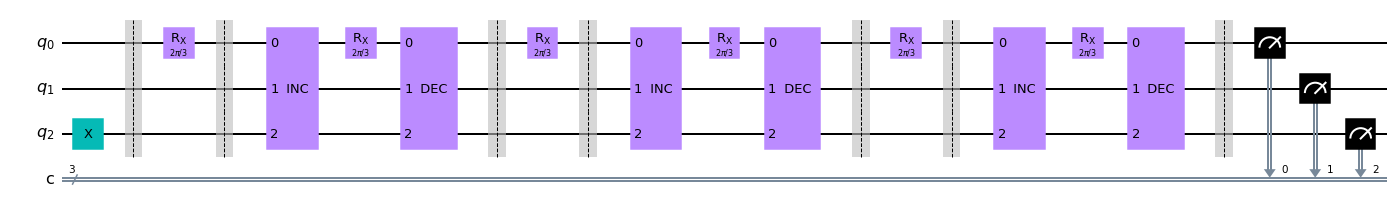
\includegraphics[scale=0.30]{img/Qiskit/StaggeredQW/Circuits/circStagQW_N3_S3.png}
	\caption{Qiskit circuit for the staggered quantum walk, for a line graph of size $N=8$ and initial condition $\ket{\psi_0}=\ket{4}$, with $3$ steps.} 
	\label{fig:stagQWCircuitQistkit}
\end{figure}
The circuit starts with a Pauli-X gate in the third qubit so that $\ket{\psi_0}
= \ket{4}$. The following operation is a rotation in the X basis, where $\theta
= \frac{\pi}{3}$, since it was seen in figure \ref{fig:stagQWSimulMultTheta}
that this value of $\theta$ maximizes the propagation of the walk. Finally,
$U_\beta$ is applied, making use of the increment and decrement gates defined
in figure \ref{fig:qiskitShiftOperator}. Note
that now, because this model does not require a coin, these gates do not need
to be controlled, meaning that the largest multi-controlled NOT gate will not
be needed, making the circuit more NISQ-friendly. This procedure is repeated
$3$ times, and the resulting probability distributions after measurement are depicted in figure \ref{fig:stagQWQiskitDist}. 
\begin{figure}[!h]
	\centering
	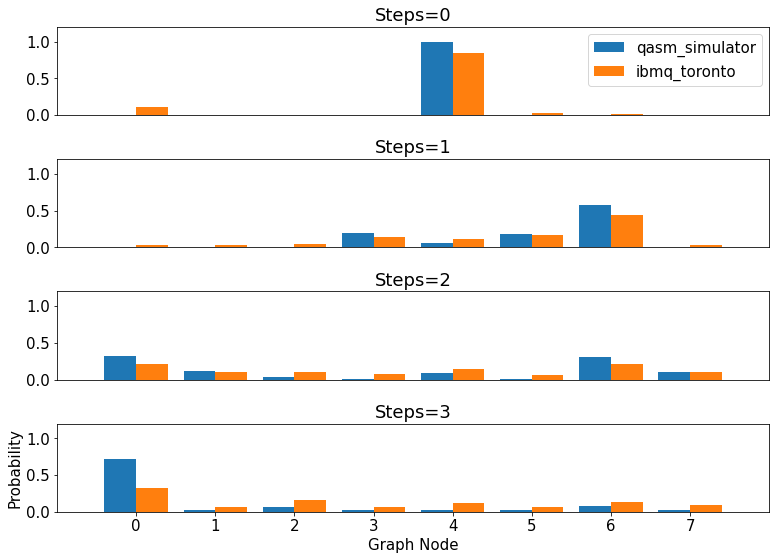
\includegraphics[scale=0.40]{img/Qiskit/StaggeredQW/StagQW_N3_S0123.png}
	\caption{Probability distributions of the staggered quantum walk for several steps in a line graph of size $N=8$. The blue bar plot represents a circuit run in the QASM simulator, and the orange bar plot on IBM's Toronto backend.} 
	\label{fig:stagQWQiskitDist}
\end{figure}\par
Analyzing the figure, it is clear that this model is much better suited for
running in current NISQ hardware. Even though the probability distribution
was somewhat affected by noise, the dynamics of the walk is relatively
unaffected in the Toronto backend experiment. This is mainly due to the much smaller number of CNOT gates, when compared to the last model. Now, for $1$, $2$ and $3$ steps, the gate count was $21$, $37$ and $64$, respectively.
\par The highest fidelity was
achieved for $2$ steps, with a value of approximately $0.95$, and the remaining
steps ranging from $0.91$ to $0.92$.  Again, it may seem counter-intuitive that
a higher fidelity is achieved for a larger circuit, compared to $0$ steps for
example, but this is again due to the balance of circuit size and spread of the
probability distribution.\par

Nevertheless, because this discrete model requires ever more operations with
the increase of steps, it will eventually become intractable for NISQ
technology. This justifies that the next model studied in this work is one where
the circuit will be constant in time.

\end{document}
